The main idea behind making bikes publicly available is for people to use them. To increase the usage we have rethought the current system and found some areas which could be improved (see \ref{errorsInOldSystem}).
We have improved the current system in these areas:
\begin{itemize}
\item The bikes have become smarter.
\item The stations have been shut down.
\item The payment and payment method have been /*changed*/
\item We have drastically increased functionality.
\end{itemize}

\subsection{The bikes}
The current bikes sometimes vanish or are left in a ditch somewhere until another user sees it and reports it. In order to enhance this method and to increase overall functionality, we have installed GPSs in all bikes. This would allow us to always keep track of the bikes and thereby allow for more features and functionality.

In order to implement some of the features we want, we needed a special lock, which could be unlocked by a keypad (see \ref{lock}). The lock should also be connected to the Internet in order for us to know when a bike is locked. It is important that the bikes are now able to be locked remotely, to ensure the safety of the user.

The lock should also be able to change its lock code every X minutes. This features ensures 

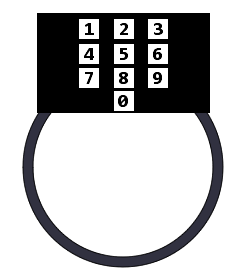
\includegraphics[width=.75\textwidth]{lock}

\subsection{The stations}
To achiever greater freedom of use we have decided to shut down the current stations. This allows the user to park the bike wherever he/she wants, and is no longer confined to the stations. This would however make it more difficult to find a bike, which is why we have implemented counter features which is described later in the report (see \ref{bikeNearby}).

\subsection{Payment}
Given that the bikes have become smarter and therefore more expensive we have decided to charge for the fares. The prices should be over time with the price increasing every increment of time.\alexander{Write precise time and price instead when decided.}
The price increase over time should solve the problem of people lending a bike and locking it with their own lock, to keep others from using it. \alexander{Source to problem?}

Payment should be done through a smartphone application or established payment-stations for those who do not have a smartphone. It should therefore not impact the usage of tourists and people without smartphones.
It is intended to work by the smartphone or payment-station grants you a position to a bike and a code which can unlock the bike for the next X minutes. This way it will not be a problem to locate the bikes, nor can a user occupy a bike without using it more than X minutes. The distance from the payment-station or smartphone to the bike should be calculated to ensure it is possible to walk to and unlocking the bike before the unlocking code changes.
\alexander{What if a user has paid through payment-station and uses the bike more than paid fore?}


\subsection{Software}
\subsubsection{Webservice}
\subsubsection{Agent}
\subsubsection{PhoneApp - Not making}
\subsubsection{PC Program - Not making}
\subsubsection{DemoProgram - making}